\documentclass[a0paper,portrait]{baposter}

\usepackage{wrapfig}
\usepackage{lmodern}
\usepackage{lipsum}

\usepackage[utf8]{inputenc} %unicode support
\usepackage[T1]{fontenc}


\selectcolormodel{cmyk}

\graphicspath{{figures/}} % Directory in which figures are stored


\newcommand{\compresslist}{%
\setlength{\itemsep}{0pt}%
\setlength{\parskip}{1pt}%
\setlength{\parsep}{0pt}%
}

\newenvironment{boenumerate}
  {\begin{enumerate}\renewcommand\labelenumi{\textbf\theenumi.}}
  {\end{enumerate}}



\begin{document}


\definecolor{pimsblue}{cmyk}{1.0,0.44,0,0}
\definecolor{lightblue}{cmyk}{0.8,0,0.25,0.8}

\begin{poster}
{
grid=false,
headerborder=open, % Adds a border around the header of content boxes
colspacing=1em, % Column spacing
bgColorOne=white, % Background color for the gradient on the left side of the poster
bgColorTwo=white, % Background color for the gradient on the right side of the poster
borderColor=lightblue, % Border color
headerColorOne=pimsblue, % Background color for the header in the content boxes (left side)
headerColorTwo=pimsblue, % Background color for the header in the content boxes (right side)
headerFontColor=white, % Text color for the header text in the content boxes
boxColorOne=white, % Background color of the content boxes
textborder=rounded, %rectangle, % Format of the border around content boxes, can be: none, bars, coils, triangles, rectangle, rounded, roundedsmall, roundedright or faded
eyecatcher=false, % Set to false for ignoring the left logo in the title and move the title left
headerheight=0.11\textheight, % Height of the header
headershape=rounded, % Specify the rounded corner in the content box headers, can be: rectangle, small-rounded, roundedright, roundedleft or rounded
headershade=plain,
headerfont=\Large\textsf, % Large, bold and sans serif font in the headers of content boxes
%textfont={\setlength{\parindent}{1.5em}}, % Uncomment for paragraph indentation
linewidth=2pt % Width of the border lines around content boxes
}
{}
%
%----------------------------------------------------------------------------------------
%	TITLE AND AUTHOR NAME
%----------------------------------------------------------------------------------------
%
{
\textsf %Sans Serif
{Title Of Your VXML Project}
} % Poster title
{\sf\vspace{0.5em}\\
Faculty Mentor\textsuperscript{1},
Graduate Mentor\textsuperscript{2},
Undergraduate Student 1\textsuperscript{3}, \ldots
\vspace{0.1em}\\
\small{1: University 1, 2: University 2, 3: University 3
\vspace{0.2em}\\
contact-email@example.com}
}
{
\includegraphics[width=0.3\linewidth]{logo}} % University/lab logo


\headerbox{1. Introduction}{name=introduction,column=0,row=0, span=3}{
\lipsum[1-1]
}


\headerbox{2. Challenges Faced}{name=challenges,column=0,below=introduction,span=1}{

\lipsum[2-2][1-3]

\begin{center}
    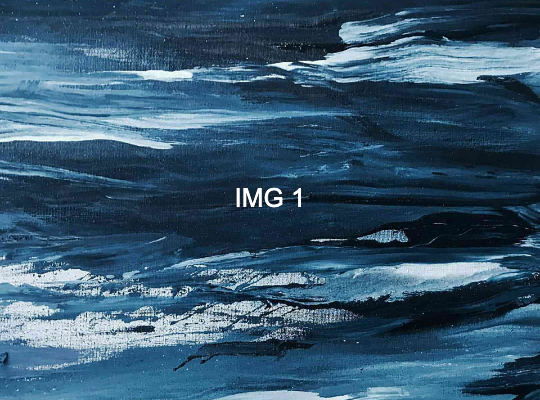
\includegraphics[width=0.6\linewidth]{1.png}
\end{center}
}


\headerbox{3. Approach}{name=approach,column=0,below=challenges,span=1}{

\lipsum[3-3][1-3]

\begin{center}
    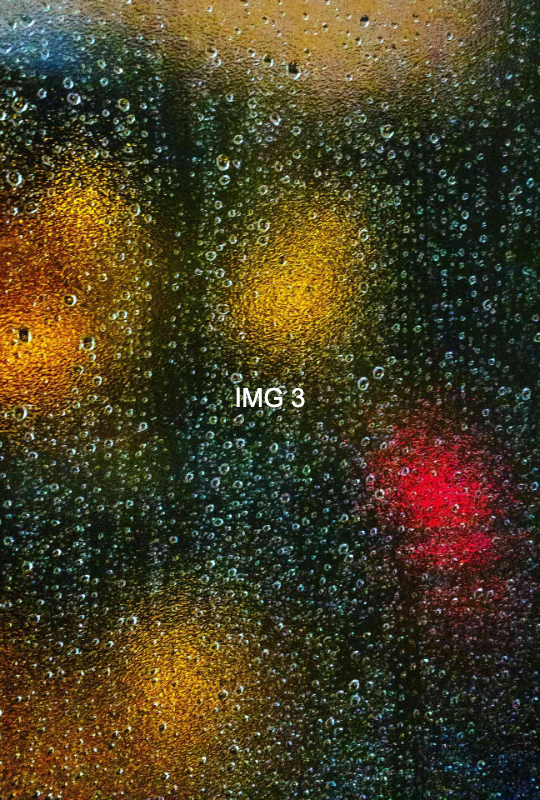
\includegraphics[width=0.7\linewidth]{3}
\end{center}
}

\headerbox{4. Results}{name=results,span=2,column=1,below=introduction}{ % To reduce this block to 1 column width, remove 'span=2'

\lipsum[5-5][1-2]
\begin{displaymath}
    \sum_{n=1} \frac{1}{n^2} = \frac{\pi^2}{6}
\end{displaymath}
\lipsum[5-5][3-3]

\vspace{-5pt}
\begin{center}
    
\includegraphics[width=0.8\linewidth]{2.png}
\end{center}
}


\headerbox{5. Conclusions}{name=conclusions,span=2,column=1,below=results}{ % To reduce this block to 1 column width, remove 'span=2'

\begin{wrapfigure}{l}{0.3\textwidth}
    \vspace{10pt}
    \begin{center}
        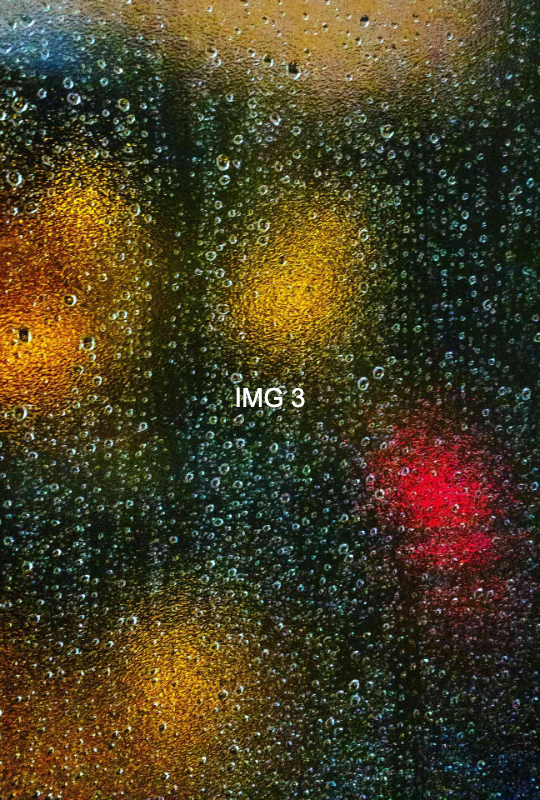
\includegraphics[width=\linewidth]{3.png}
    \end{center}
    %\vspace{-145pt}
\end{wrapfigure}

\lipsum[6-6][1-4]

\hspace{160pt}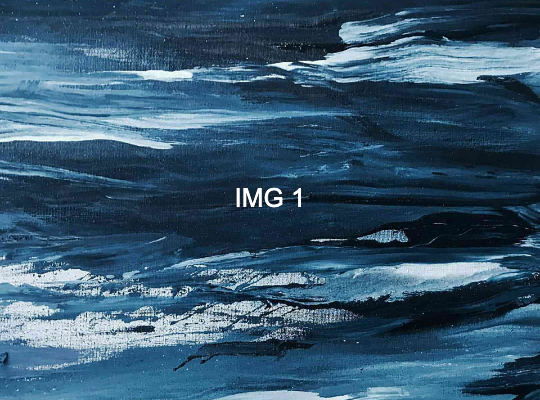
\includegraphics[width=0.85\linewidth]{1.png}

}


\headerbox{6. Future Directions}{name=conclusions,column=1,below=conclusions,span=2,above=bottom}{
\begin{boenumerate}\compresslist
    \item \lipsum[8-8][1-1]
    \item \lipsum[8-8][2-2]
    \item \lipsum[8-8][3-3]
\end{boenumerate}
}


\headerbox{7. References}{name=references,column=0,span=1,below=approach,above=bottom}{


%\small % Reduce the font size in this block
\renewcommand{\section}[2]{\vskip 0.05em} % Get rid of the default "References" section title
%\nocite{*} % Insert publications even if they are not cited in the poster


\bibliographystyle{unsrt}
\begin{thebibliography}{9}
\bibitem{lamport94}
  Leslie Lamport,
  \textit{\LaTeX: a document preparation system},
  Addison Wesley, Massachusetts,
  2nd edition,
  1994.
\bibitem{texbook}
  Donald Ervin Knuth.
  \textit{The \TeX book}.
  Addison-Wesley, Reading, Massachusetts, 1983.
\end{thebibliography}
}

\end{poster}

\end{document}
